\subsection{Choosing the next wave}\label{cc:uf:sec:later-wave}
Let $U$ and its flow $X$ be as in Subsection~\ref{cc:uf:sec:parent-step}.
The new wave starts at $t_0$ with frequency $\lambda$. The origin is a
fixed particle. Once the preceding wave's cutoff
equals one, \eqref{cc:uf:tower:eq:central-return} and the truncation
estimate \eqref{cc:uf:step:eq:truncated} give its contribution to the
gradient there. Suppose, accordingly, that on $[t_0,T]$ the gradient
$M=\nabla U(t,0)$ has the form
\begin{equation}\label{cc:uf:tower:eq:split}
 M=B+\mathbf a_p\otimes\kappa_p+E_c ,
\end{equation}
where $B$ is the smooth trace-free gradient of the older velocity, $(\mathbf a_p,\kappa_p)$ is
the preceding wave over $B$, and $E_c$ contains the errors from its
corrections and truncation. The preceding pair solves
\eqref{cc:eq:wave-ode} with $D=B$. In its moving frame $(E_i)$ write
$B_{ij}=E_i\cdot BE_j$. At $t_0$ freeze its strength
$\sigma=|\mathbf a_p||\kappa_p|$ and its couplings $\nu=B_{12}>0$ and
$\eta=B_{32}>0$. As in Subsection~\ref{cc:sec:comparison}, put
$r=\sqrt{2\sigma\nu}$, $S=\sigma/r$, $\varepsilon=\eta/\nu$ and
$\tau=r(t-t_0)$.

Choose the wave vector at activation perpendicular to the preceding
wave vector and amplitude. Since $\kappa=(D_aX)^{-T}k_*$, the
time-zero vector that gives $\kappa(t_0,0)=\lambda E_3(t_0)$ is
\[
 k_*=\lambda (D_aX(t_0,0))^TE_3(t_0).
\]
For the amplitude take the growing direction
$-E_1(t_0)/S+E_2(t_0)$. In the coordinates of \eqref{cc:eq:scaled-pair}
this is $(U,V)=(1,1)$ at $\tau=0$. Scale the seed by a positive
constant so that $\max_{[t_0,T]}|\mathbf a(t,0)|=\lambda^{-3/4}$, and
write $\gamma(t)=\lambda^{3/4}|\mathbf a(t,0)|$ as in
Subsection~\ref{cc:uf:sec:parent-step}.

To apply the comparison of Subsection~\ref{cc:sec:amplification}, we need
to bound the variation of the two couplings of $B$ in the moving frame.
When $\varepsilon\le1$, the comparison error
\eqref{cc:uf:exact:eq:additive-error} satisfies
\begin{equation}\label{cc:uf:tower:eq:active-error}
 \delta\le C\left[
 \frac{(T-t_0)\bigl(\norm B_\infty^2+\norm{B_t}_\infty\bigr)}{\eta}
 +\frac{\norm B_\infty}{r}+\frac{\norm{E_c}_\infty}{\nu}\right].
\end{equation}
Here the suprema are over $[t_0,T]$. Indeed, the frame equations
\eqref{cc:eq:frame} give $|\partial_t E_i|\le2\norm B_\infty$, so
$|\partial_t B_{ij}|\le4\norm B_\infty^2+\norm{B_t}_\infty$.
Integration from $t_0$ bounds the changes in $B_{12}$ and $B_{32}$.
Dividing by their frozen values $\nu$ and $\eta$, with $\eta\le\nu$,
gives the first term of \eqref{cc:uf:tower:eq:active-error}. The other
two terms occur directly in \eqref{cc:uf:exact:eq:additive-error}.

Suppose the normalized interval has length $r(T-t_0)\ge2$ and that
\eqref{cc:eq:finite-smallness} holds with this length in place of $T$.
Lemma~\ref{cc:lem:finite-comparison} then applies to the chosen
direction. The positive rescaling of the seed preserves its frame and
all ratios of its lengths. Write $\nu_+,\eta_+$ for the couplings of
$M$ in the frame of the new wave. For $t_0\le t'\le t\le T$ and every
transverse solution $\mathbf b$ of the seed equation at the origin,
the lemma gives
\begin{equation}\label{cc:uf:tower:eq:later-origin}
 \frac{|\mathbf b(t)|}{\gamma(t)}
 \le CS\,\frac{|\mathbf b(t')|}{\gamma(t')},\qquad
 \nu_+(t)\ge\tfrac12\nu\varepsilon.
\end{equation}
These are the two estimates \eqref{cc:uf:tower:eq:wave-origin} when
$\mathsf D$ bounds $CS$ and $2/(\nu\varepsilon)$.

We switch on the wave during the first unit of normalized time. With
the function $\chi$ of Subsection~\ref{cc:uf:sec:parent-step}, take
\[
 \widetilde\chi(t)=1-\chi\bigl(1+r(t-t_0)\bigr)\quad(t\ge t_0),\qquad
 \widetilde\chi(t)=0\quad(t<t_0).
\]
This cutoff is smooth, equals one for $\tau\ge1$ and satisfies
$|\widetilde\chi'|\le Cr$. Prescribe the coupling ratio
$0<\varepsilon_+\le\varepsilon/32$ for the following wave, and suppose
$r(T-t_0)\ge2(\varepsilon\varepsilon_+)^{-1/2}$. By \eqref{cc:eq:gain},
\begin{equation}\label{cc:uf:tower:eq:switch-small}
 \gamma\le\exp\bigl(3-\varepsilon^{-1/2}\bigr)
 \qquad\hbox{on }[t_0,t_0+1/r].
\end{equation}
Thus the factor $\|\widetilde\chi'\gamma\|_\infty$ in the residual
estimate \eqref{cc:uf:step:eq:physical} is at most
$Cr\exp(3-\varepsilon^{-1/2})$.

Proposition~\ref{cc:prop:finite-return} also gives a time in
$\tau_m\le\tau\le2(\varepsilon\varepsilon_+)^{-1/2}$ at which
$\eta_+/\nu_+=\varepsilon_+$. We activate the following wave at the
first such crossing in this interval. Since the reference amplitude
peaks at $\tau_m\ge2/\varepsilon>1$, the cutoff already equals one
there, and \eqref{cc:eq:general-return} gives the strength of the
shear available to amplify that wave.

\section{A common sequence of approximate solutions}\label{cc:uf:sec:tower}

We construct a single sequence of approximate solutions for all
derivative orders. The parent for wave $1$ is the stationary shear
\eqref{cc:uf:base:eq:stationary} with $s=\varepsilon_1$. At step $j$
we choose the wave over $U_{j-1}$ as in Section~\ref{cc:sec:iteration}
and apply Proposition~\ref{cc:uf:step:thm:step} to obtain $U_j$.
The frequencies and orders are fixed by \eqref{cc:uf:tower:eq:schedule}.
The residual of $U_j$ must already be small on the scale of the
frequency $\lambda_{j+1}$ of the next wave.

Write $X_j$ for the flow of $U_j$ from time zero, and $\pi_j$ and $R_j$
for its pressure and its residual, defined as $p_U$ and $R_U$ are for
the parent in Subsection~\ref{cc:uf:sec:parent-step}.
At the center, let $\mathbf a_j,\kappa_j,\sigma_j$ be the seed,
wave vector and strength of wave $j$, and let
\begin{equation}\label{cc:uf:tower:eq:couplings}
 \nu_j=\frac{\kappa_j}{|\kappa_j|}\cdot\nabla U_{j-1}(t,0)
        \frac{\mathbf a_j}{|\mathbf a_j|},\qquad
 \eta_j=\frac{\kappa_j\times\mathbf a_j}{|\kappa_j||\mathbf a_j|}
        \cdot\nabla U_{j-1}(t,0)\frac{\mathbf a_j}{|\mathbf a_j|}
\end{equation}
be the couplings of $\nabla U_{j-1}(t,0)$ in the frame of this pair.
For $j\ge2$ these are $\nu_+,\eta_+$ of Subsection~\ref{cc:uf:sec:later-wave}.
Let $\widetilde\chi_j$ be the time cutoff of wave $j$ and
$O_j=W_{\rm osc}^\natural$ its oscillatory velocity increment before
truncation, as in Lemma~\ref{cc:uf:step:lem:approximate}.

The first two waves start at time zero. Given the activation time $t_j$,
we fix the final time $S_j$ of the endpoint equations by
\[
 t_1=t_2=0,\qquad
 \tau_j=\lambda_{j-1}^{-1/8}L_{j+1}^3,\qquad
 S_0=1,\qquad S_j=t_j+2\tau_j\quad(j\ge1).
\]
For $j\ge2$ we normalize the seed on $[t_j,S_j]$. The central wave
equations over $U_{j-1}$ then determine $t_{j+1}$ on that interval.
We take the first crossing
of $\eta_j/\nu_j=\varepsilon_j$ in the interval of
Proposition~\ref{cc:prop:finite-return}. It will occur by $t_j+\tau_j$,
leaving room before $S_j$ for the subsequent activation times.
To make the remainder of the expansion small at frequency $\lambda_{j+1}$,
we take the depth
\begin{equation}\label{cc:uf:tower:eq:step-orders}
 P=6K_{j+1}.
\end{equation}

\Needspace{8\baselineskip}
\begin{theorem}\label{cc:uf:tower:thm:finite}
For every sufficiently large $N$ there are fields $U_j$, $j\ge1$, and
times $0=t_1=t_2<t_3<\cdots$ with the following properties, in which
$U_0$ is the shear \eqref{cc:uf:base:eq:stationary} at $s=\varepsilon_1$:
\textup{(T1)}--\textup{(T3)} for $j\ge0$ and \textup{(T4)} for $j\ge1$.
\begin{enumerate}[label=(T\arabic*),leftmargin=*]
\item $U_j$ is a smooth odd divergence-free field on
$[0,S_j]\times\mathbb T^3$, supported on frequencies at most $2\Lambda_j$.
\item $\norm{U_j}_{C_tL^\infty}\le\lambda_j$,
$\sup|(D_aX_j)^{\pm1}|\le\lambda_j$ and
$\norm{R_j}_{C_tL^\infty}\le\lambda_{j+1}^{-3}$.
\item $D^2\pi_j\le\bigl(\sum_{i=1}^j\lambda_{i-1}^{-1}\bigr)\Id$ on
$[0,S_j]\times\mathbb T^3$.
\item At the center on $[t_j,S_j]$,
$\nabla U_j=\nabla U_{j-1}
+\widetilde\chi_j\,\mathbf a_j\otimes\kappa_j+E_{c,j}$ with
$|E_{c,j}|\le\lambda_j^{-1/4}$. Moreover
$0\le t_{j+1}-t_j\le\tau_j$ and $\widetilde\chi_j=1$ on
$[t_{j+1},S_j]$, so that the gradient of $U_j$ has the splitting
\eqref{cc:uf:tower:eq:split} there. At $t_{j+1}$, with an absolute
constant $C\ge2$ for which \eqref{cc:eq:general-return} holds,
\begin{equation}\label{cc:uf:tower:eq:late-values}
 \frac{\eta_j}{\nu_j}=\varepsilon_j,\qquad
 \pi\le\nu_j\le4\pi,\qquad
 C^{-1}\lambda_j^{1/4}\le\sigma_j\le C\lambda_j^{1/4}L_{j+1}^2 .
\end{equation}
\end{enumerate}
The activation times converge to a limit
$T_\infty\in(0,\infty)$, and $T_\infty<S_j$ for every $j$. For $j\ge1$
the oscillation $O_j$ is supported, at each time of $[0,S_j]$, in the
ball of radius $\lambda_{j-1}^{-1}$ about the origin, and
\begin{equation}\label{cc:uf:tower:eq:increment}
 \|O_j\|_{C([0,S_j];L^\infty)}\le\lambda_j^{-1},\qquad
 \|U_j-U_{j-1}-O_j\|_{C([0,S_j];\Holder{m})}\le\lambda_j^{-1}
 \quad(0\le m\le q_j).
\end{equation}
For $j\ge2$ the oscillation $O_j$ vanishes on $[0,t_j]$.
\end{theorem}

For each fixed $m$, the orders $q_j$ eventually exceed $m$. By
\eqref{cc:uf:tower:eq:increment}, the increments $U_j-U_{j-1}-O_j$
are then summable in $\Holder{m}$ on the common interval $[0,T_\infty]$.
On $[0,t_j]$ they give the entire velocity increment for $j\ge2$.
This is the estimate used for convergence in
Section~\ref{cc:sec:limit}. Figure~\ref{cc:fig:construction-timeline}
shows the intervals on which the oscillations are present.

\begin{figure}[!htbp]
\centering
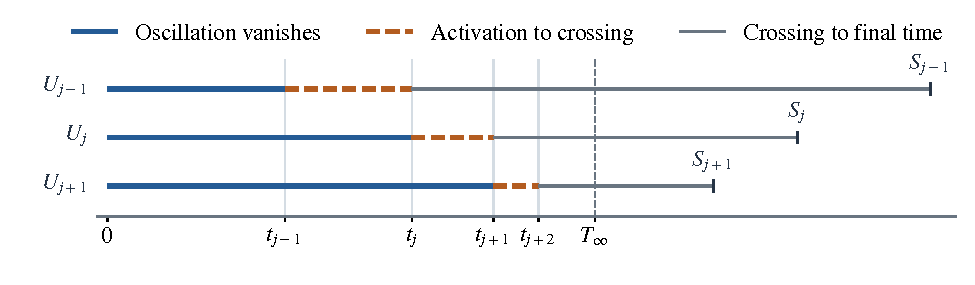
\includegraphics[width=\textwidth]{figures/construction-timeline.pdf}
\caption{Three successive approximate solutions for $j\ge4$. In each row
the oscillation vanishes on the thick solid segment $[0,t_i]$. The
dashed segment ends at the crossing $t_{i+1}$, when the next wave is
activated. Each solution continues to its final time $S_i>T_\infty$.}
\label{cc:fig:construction-timeline}
\end{figure}

\subsection{The data of a step}

At any index $j$ for which \textup{(T1)} and \textup{(T2)} hold, the
frequency bound gives estimates for the gradient and its time derivative.
As in Subsection~\ref{cc:uf:sec:parent-step}, the residual is supported
on frequencies at most $4\Lambda_j$ and
\begin{equation}\label{cc:uf:tower:eq:leray}
 \partial_tU_j=-\PP\diver(U_j\otimes U_j)+R_j .
\end{equation}
By \eqref{cc:uf:trunc:eq:lp},
$\|\nabla U_j\|_\infty\le C\Lambda_j\lambda_j$ and
$\|\nabla R_j\|_\infty\le C\Lambda_j\lambda_{j+1}^{-3}$.
For the time derivative of the gradient, apply \eqref{cc:uf:trunc:eq:lp}
to $U_j\otimes U_j$ and use the boundedness of $\PP$ on $\Holder{0}$
in \eqref{cc:uf:tower:eq:leray}. Two spatial derivatives of the product
in $\Holder{0}$ cost at most $C\Lambda_j^3\lambda_j^2=C\lambda_j^{17}$.
Thus for large $N$,
\begin{equation}\label{cc:uf:tower:eq:derived-low}
 \|\nabla U_j\|_\infty\le\lambda_j^9,\qquad
 \|\partial_t\nabla U_j\|_\infty\le\lambda_j^{18}
 \quad\hbox{on }[0,S_j].
\end{equation}
At step $j$ we apply Section~\ref{cc:sec:exact} with $U=U_{j-1}$,
$\lambda=\lambda_j$, activation time $t_j$ and final time $S_j$. Write
$\mu=\lambda_{j-1}$ and $\widetilde\chi=\widetilde\chi_j$. By
\eqref{cc:uf:tower:eq:derived-low} at $j-1$ we can take
$\mathsf D=\mu^9$ for the parent gradient. When $j\ge2$ we also use
\eqref{cc:uf:tower:eq:derived-low} at $j-2$ for the older gradient in
the wave comparison. The final Fourier cutoff is $\Lambda_j=\lambda^5$.

To compare successive final times, observe that by \eqref{cc:uf:tower:eq:uniform},
$\tau_j=\mu^{-1/8}L_{j+1}^3\le\mu^{-1/16}$ for large $N$.
Applying this bound at $j+1$ and using $\lambda_j\ge\mu^4$ gives
$4\tau_{j+1}\le4\mu^{-1/4}\le\mu^{-1/8}\le\tau_j$. Thus
\begin{equation}\label{cc:uf:tower:eq:increment-tail}
 \tau_j\le\lambda_{j-1}^{-1/16},\qquad 4\tau_{j+1}\le\tau_j ,
\end{equation}
uniformly in $j$ for large $N$.

Finally the depth $P=6K_{j+1}$ in \eqref{cc:uf:tower:eq:step-orders}
requires estimates through order $P+1$. Since $P+1\le7K(q_{j+1})$,
$\mathcal B(q_{j+1})$ bounds all the fixed-order constants used in
Section~\ref{cc:sec:exact} and Lemma~\ref{cc:uf:trunc:lem:cutoff}
at these orders and this depth.
The choice of $q_{j+1}$ in \eqref{cc:uf:tower:eq:schedule} gives
$\mathcal B(q_{j+1})\le\mu$. With $\mathsf D=\mu^9$ and
$\lambda=\mu^{K_j}$, $K_j=320b(q_j+1)$, we obtain
\begin{equation}\label{cc:par:step}
 \mathcal B(q_{j+1})\mathsf D^b\le\mu^{10b}\le\lambda^{1/32}.
\end{equation}

\subsection{Proof of Theorem~\ref{cc:uf:tower:thm:finite}}

For $j=0$, the shear $U_0$ has only the Fourier modes $\pm e_2$,
$\|U_0\|_\infty\le2$, and its pressure and residual vanish. Its
deformation and inverse have norm at most $1+4\pi$ on $[0,S_0]$
by \eqref{cc:uf:base:eq:deformation}. These give \textup{(T1)}--\textup{(T3)}
for large $N$.

Suppose the construction has been carried out through step $j-1$.
For $j=1$, \eqref{cc:uf:tower:eq:increment-tail} gives
$S_1=2\tau_1\le S_0=1$. For $j\ge2$, the previous crossing occurred
by $t_{j-1}+\tau_{j-1}$. Since $2\tau_j\le\tau_{j-1}/2$,
\[
 S_j=t_j+2\tau_j\le t_{j-1}+\tfrac32\tau_{j-1}<S_{j-1}.
\]
Thus $U_{j-1}$ is available on the entire interval $[0,S_j]$ of
the endpoint problem.

\begin{enumerate}[leftmargin=*]
\item \emph{Estimates for the parent.}
On $[0,S_j]\subset[0,S_{j-1}]$, (T1) bounds the frequencies of $U=U_{j-1}$
by $2\Lambda_{j-1}=2\mu^5\le2\mathsf D$. By (T2) and
\eqref{cc:uf:tower:eq:derived-low}, $\sup|(D_aX)^{\pm1}|\le\mu$ and
$\|\nabla U\|_\infty\le\mu^9=\mathsf D$, as required in
\eqref{cc:uf:tower:eq:parent-bound}. The residual bound
$\|R_{j-1}\|_{C_tL^\infty}\le\lambda^{-3}$ in (T2) gives
\eqref{cc:uf:tower:eq:parent-small}. For the endpoint problem we also need
\eqref{cc:uf:tower:eq:parent-coercive}. The derivative bound preceding
\eqref{cc:uf:tower:eq:derived-low} gives $\|\nabla R_{j-1}\|_\infty
\le C\mu^5\lambda^{-3}$. In (T3) the sum is at most $2/N$, since $\lambda_0=N$ and
$\lambda_i\ge2\lambda_{i-1}$. Thus
$D^2\pi_{j-1}-\nabla R_{j-1}\le(2/N+C\mu^5\lambda^{-3})\Id$
as quadratic forms, which gives \eqref{cc:uf:tower:eq:parent-coercive} for large $N$.

\item \emph{Choosing wave $j$.}
For $j=1$ take the wave \eqref{cc:uf:base:eq:first-wave} of frequency
$\lambda_1$ on $[0,S_1]$. Since $4\pi S_1\le1/8$ for large $N$,
Lemma~\ref{cc:uf:base:lem:first} gives \eqref{cc:uf:tower:eq:wave-origin}
and the strength bounds in \eqref{cc:uf:tower:eq:late-values} at
$t_2=t_1=0$. The couplings there are $\nu_1=2\pi$ and
$\eta_1=2\pi\varepsilon_1$ by \eqref{cc:uf:base:eq:shear-couplings}.
The first wave has $\widetilde\chi_1\equiv1$.

For $j\ge2$, (T4) at $j-1$ gives the splitting
\eqref{cc:uf:tower:eq:split} on $[t_j,S_j]$ with $B=\nabla U_{j-2}(t,0)$,
the preceding pair $(\mathbf a_{j-1},\kappa_{j-1})$ and
$\|E_c\|_\infty\le\mu^{-1/4}$. The pair solves \eqref{cc:eq:wave-ode}
over $B$ because the flow of $U_{j-2}$ fixes the origin. Freeze its
couplings and strength at $t_j$. For $j=2$ these are the values of
wave~$1$ at time zero. For $j\ge3$ they are the values at the preceding crossing.
In both cases \eqref{cc:uf:tower:eq:late-values} gives
\[
 \varepsilon=\varepsilon_{j-1}=L_j^{-2},\qquad
 \pi\le\nu\le4\pi,\qquad
 c\mu^{1/4}\le\sigma\le C\mu^{1/4}L_j^2 .
\]
Choose the wave of Subsection~\ref{cc:uf:sec:later-wave}, whose wave
vector has length $\lambda$ at $t_j$. Since $r=\sqrt{2\sigma\nu}$,
$c\mu^{1/8}\le r\le C\mu^{1/8}L_j$. The normalized length
$r(S_j-t_j)=2r\mu^{-1/8}L_{j+1}^3$ is therefore between $2$ and
$CL_{j+1}^4$ for large $N$.

To check the comparison on this interval, \eqref{cc:uf:tower:eq:derived-low}
at $j-2$ gives $\|B\|_\infty\le\lambda_{j-2}^9\le\mu^{1/32}$ and
$\|B_t\|_\infty\le\mu^{1/16}$, since $\lambda_{j-2}=\mu^{1/K_{j-1}}$
and $K_{j-1}>288$. With $\eta=\nu\varepsilon$, the three terms in
\eqref{cc:uf:tower:eq:active-error} give
\[
 \delta\le C\bigl(\varepsilon^{-1}L_{j+1}^3\mu^{-1/16}
                   +\mu^{-3/32}+\mu^{-1/4}\bigr).
\]
By \eqref{cc:uf:tower:eq:uniform}, $L_j\le L_{j+1}\le(\log\mu)^2$.
Thus $C_0(2r\tau_j)^{C_0}\delta/\varepsilon$ is bounded by
$\mu^{-1/16}$ times a fixed power of $\log\mu$, and
$C_0\varepsilon\le C_0(\log N)^{-2}$. For large $N$ both conditions
of \eqref{cc:eq:finite-smallness} hold. In the resulting central estimates
\eqref{cc:uf:tower:eq:later-origin}, $CS=Cr/(2\nu)\le C\mu^{1/8}L_j$
and $2/(\nu\varepsilon)\le 2L_j^2/\pi$. Both are at most $\mu\le\mathsf D$
for large $N$. This proves \eqref{cc:uf:tower:eq:wave-origin} for wave $j$.

\item \emph{The next activation time.}
For $j\ge2$ we seek a crossing with $\eta_j/\nu_j=\varepsilon_j$ in
the first half of $[t_j,S_j]$. Then $t_{j+1}\le t_j+\tau_j$ leaves
room for the next interval, since $2\tau_{j+1}\le\tau_j/2$ by
\eqref{cc:uf:tower:eq:increment-tail}. The schedule
\eqref{cc:uf:tower:eq:schedule} gives $L_{j+1}/L_j=K_{j+2}\ge640$, so
\begin{equation}\label{cc:uf:tower:eq:ratio}
 \varepsilon_j=(L_j/L_{j+1})^2\varepsilon_{j-1}\le\varepsilon_{j-1}/32,
\end{equation}
and $(\varepsilon\varepsilon_j)^{-1/2}=L_jL_{j+1}\le L_{j+1}^2$.
In physical time the upper endpoint of the bracket in
Proposition~\ref{cc:prop:finite-return} lies at most $\tau_j$ after $t_j$. Indeed,
\[
 \frac{2(\varepsilon\varepsilon_j)^{-1/2}}{r}
 \le C\mu^{-1/8}L_{j+1}^2\le\tau_j ,
\]
using $r\ge c\mu^{1/8}$ and $L_{j+1}\ge\log N$. Take $t_{j+1}$ to be
the first crossing in that interval. Its normalized time is at least
$\tau_m\ge2/\varepsilon>1$, so $0<t_{j+1}-t_j\le\tau_j$ and
$\widetilde\chi=1$ on $[t_{j+1},S_j]$.

At this crossing \eqref{cc:eq:general-return} bounds $\sigma_j(t_{j+1})$
above and below by absolute multiples of $\lambda^{1/4}L_jL_{j+1}$,
since $\max_{[t_j,S_j]}|\mathbf a_j(t,0)|=\lambda^{-3/4}$.
As $1\le L_jL_{j+1}\le L_{j+1}^2$, this gives the strength bounds in
\eqref{cc:uf:tower:eq:late-values}. Equation~\eqref{cc:eq:actual-ratio}
applies at the same time and gives
\[
 \bigl|\log\bigl(\nu_j(t_{j+1})/\nu_{j-1}(t_j)\bigr)\bigr|
 \le2\varepsilon_{j-1}.
\]
Summing this inequality over the successive crossings from
$\nu_1(t_2)=2\pi$ and using
$\varepsilon_i\le32^{1-i}\varepsilon_1$ from \eqref{cc:uf:tower:eq:ratio}
gives $|\log(\nu_j(t_{j+1})/(2\pi))|\le4\varepsilon_1\le4(\log N)^{-2}$.
Thus $\pi\le\nu_j(t_{j+1})\le4\pi$ for large $N$, completing
\eqref{cc:uf:tower:eq:late-values}.

On the interval where the cutoff changes, \eqref{cc:uf:tower:eq:switch-small}
gives $\gamma\le e^{3-L_j}=e^3\lambda_{j+1}^{-4}$. Since
$|\widetilde\chi'|\le Cr$ and $Ce^3r\le\mu$ for large $N$ by item~2,
\begin{equation}\label{cc:uf:tower:eq:switch-induction}
 \|\widetilde\chi'\gamma\|_\infty\le\mu\lambda_{j+1}^{-4}.
\end{equation}
The same estimate holds for the first wave since $\widetilde\chi_1'\equiv0$.

\item \emph{The expansion and its truncation.}
Items 1 and 2 give the parent and wave assumptions of
Subsection~\ref{cc:uf:sec:parent-step}. By \eqref{cc:par:step},
$C_{\rm step}=\Gamma_P\mathsf D^b\le\mu^{10b}\le\lambda^{1/32}$,
so \eqref{cc:uf:step:eq:small} holds. We can therefore apply the
expansion and truncation estimates of Section~\ref{cc:sec:exact}.

The new residual must be small at the frequency $\lambda_{j+1}$ of the
next wave. For the expansion remainder, the depth
\eqref{cc:uf:tower:eq:step-orders} gives
$\lambda^{-2P/3}=\lambda^{-4K_{j+1}}=\lambda_{j+1}^{-4}$.
For the time cutoff, item 3 gives the bound
\eqref{cc:uf:tower:eq:switch-induction}, with the same decay up to a factor $\mu$. Thus
\eqref{cc:uf:step:eq:physical} and $C_{\rm step}\mu\le\lambda^{1/16}$ give
\begin{equation}\label{cc:uf:tower:eq:frequency}
 \norm{R_V}_{C_t\Holder{1}}\le2\lambda^{2+1/16}\lambda_{j+1}^{-4}
 \le\lambda_{j+1}^{-7/2}.
\end{equation}

To estimate the Fourier tail in \eqref{cc:uf:step:eq:truncation}, we
need $\norm V_{C_t\Holder{P}}$. For the parent $U=U_{j-1}$, (T1), (T2)
and the Bernstein bound \eqref{cc:uf:trunc:eq:lp} give
$\norm U_{C_t\Holder{P}}\le C_P\mu^{5(P+1)+1}\le\lambda^{P+2}$,
since $C_P\le\mu$ and $\lambda=\mu^{K_j}$ with $K_j\ge6$.
For the wave, \eqref{cc:par:step} bounds the factor
$C_{P,P}\mathsf D^{b(P+2)}$ in \eqref{cc:uf:step:eq:physical}
by $\lambda^{(P+2)/32}$. The larger of the two resulting exponents
for the oscillation and the mean is $3P/2+1/4+(P+2)/32$.
This gives $\norm{W^\natural}_{C_t\Holder{P}}\le\lambda^{2(P+1)}$
for large $N$. Hence $1+\norm V_{C_t\Holder{P}}\le3\lambda^{2(P+1)}$.
Inserting this with $\Lambda=\lambda^5$ and $9\mu\le\lambda$ gives
\begin{equation}\label{cc:uf:tower:eq:tail-small}
 \mu\varepsilon_\Lambda\le9\mu\lambda^{5(2-P)+4(P+1)}
 \le\lambda^{15-P}
 =\lambda^{15}\lambda_{j+1}^{-6}\le\lambda_{j+1}^{-5}.
\end{equation}
In particular $C_{2,P}\varepsilon_\Lambda\le\lambda_{j+1}^{-5}$.

\item \emph{The new velocity.}
Take $U_j=S_{\Lambda_j}V$ in Proposition~\ref{cc:uf:step:thm:step}.
The proposition gives (T1), and \eqref{cc:uf:step:eq:truncated} with
\eqref{cc:uf:tower:eq:frequency} and \eqref{cc:uf:tower:eq:tail-small} gives
\[
 \norm{R_j}_{C_tL^\infty}\le C\lambda_{j+1}^{-7/2}+\lambda_{j+1}^{-5}
 \le\lambda_{j+1}^{-3},\qquad
 \norm{v_\Lambda}_{C_tC^2}\le\lambda_{j+1}^{-5}.
\]
Since $U_j=V+v_\Lambda$ and $\lambda_{j+1}^{-5}\le\lambda^{-5/2}$,
the divergence-free field $v_\Lambda$ satisfies the hypothesis of
Lemma~\ref{cc:uf:step:lem:flow-bounds}. It follows that
$\sup|(D_aX_j)^{\pm1}|\le C_{\rm step}\lambda^{1/4}\le\lambda$.

By Proposition~\ref{cc:uf:hier:prop:identity}, $W_{\rm osc}$ is supported
in $|a|\le2\ell_*$ in label coordinates. The support of
$O_j=W_{\rm osc}^\natural$ lies in the image of this ball under the
parent flow. The flow fixes the origin, so
\eqref{cc:uf:tower:eq:parent-bound} and $\ell_*\le\mathsf D^{-3}$
place its Eulerian support in the ball of radius
$2\mathsf D\ell_*\le2\mathsf D^{-2}\le\mu^{-1}$.
For $j\ge2$, $O_j$ vanishes before $t_j$ by the same proposition.
It vanishes also at $t_j$, since $\widetilde\chi(t_j)=0$ and the higher
oscillatory profiles have zero data there by Subsection~\ref{cc:uf:sec:transverse}.
By \eqref{cc:uf:step:eq:physical-sup} and \eqref{cc:par:step},
$\norm{O_j}_{C_tL^\infty}\le\lambda^{1/32}\lambda^{-5/4}\le\lambda^{-1}$.

The rest of the velocity increment can extend across the torus. Since
$V=U_{j-1}+W^\natural$,
\[
 U_j-U_{j-1}-O_j=\bar W^\natural+v_\Lambda .
\]
For $0\le m\le q_j$, the coefficient $C_{m,P}\mathsf D^{b(m+2)}$
in \eqref{cc:uf:step:eq:physical} is at most $\mu^{10b(m+2)}\le
\lambda^{1/16}$, since $K_j=320b(q_j+1)$. Thus
$\|\bar W^\natural\|_{C_t\Holder{m}}\le\lambda^{1/16-5/2}
\le\lambda^{-3/2}$. For the Fourier tail, \eqref{cc:uf:trunc:eq:tail}
at order $P$ and \eqref{cc:uf:tower:eq:tail-small} give
\[
 \|v_\Lambda\|_{C_t\Holder{m}}
 \le\mu\Lambda_j^{m-P}\norm V_{C_t\Holder{P}}
 \le\Lambda_j^{m-2}\mu\varepsilon_\Lambda
 \le\lambda^{5q_j}\lambda_{j+1}^{-5}\le\lambda_{j+1}^{-4},
\]
where $K_{j+1}\ge K_j\ge5q_j$. The sum of the mean and tail bounds is
at most $\lambda^{-1}$, proving \eqref{cc:uf:tower:eq:increment}.
In particular $\norm{U_j}_{C_tL^\infty}\le\mu+2\lambda^{-1}\le\lambda$
by (T2) for the parent. This completes (T2) for $U_j$.

\item \emph{Pressure and the central velocity gradient.}
For the pressure increment, the leading term in \eqref{cc:uf:step:eq:pressure-error}
satisfies $C_{\rm step}\lambda^{-1/4}\le\lambda^{-7/32}\le\mu^{-2}$.
By \eqref{cc:uf:tower:eq:frequency} and \eqref{cc:uf:tower:eq:tail-small},
the other two terms are at most $C\lambda_{j+1}^{-7/2}+\lambda_{j+1}^{-5}$.
Hence $D^2\pi_j\le D^2\pi_{j-1}+\mu^{-1}\Id$ on $[0,S_j]$ for large $N$.
Since $\mu^{-1}=\lambda_{j-1}^{-1}$ and $S_j\le S_{j-1}$, adding this
increment to (T3) for the parent proves (T3) at step $j$.

At the origin truncation adds $\nabla v_\Lambda(t,0)$ to the gradient
in \eqref{cc:uf:tower:eq:central-return}. Thus the new error is
$E_{c,j}=E_c+\nabla v_\Lambda(t,0)$ with
$|E_{c,j}|\le\lambda^{-1/3}+\lambda_{j+1}^{-5}\le\lambda^{-1/4}$.
From $t_{j+1}$ onward the cutoff equals one, so the full rank-one
term is present for the next wave. With the coupling and strength bounds
from items 2 and 3, this proves (T4) and closes the induction.
\end{enumerate}

The activation times increase strictly from $t_2=0$ onward. By (T4)
their successive differences are bounded by $\tau_j$, so
\eqref{cc:uf:tower:eq:increment-tail} gives a finite limit
$T_\infty\ge t_3>0$. For $j\ge1$,
\[
 0<T_\infty-t_j\le\sum_{p\ge j}\tau_p\le\tfrac43\tau_j<S_j-t_j .
\]
Thus $T_\infty<S_j$ for $j\ge1$, and $T_\infty<S_0$ since $S_1\le S_0$.
